\documentclass{article}
\usepackage[utf8]{inputenc}

\title{Homework 4 - Objects \& Classes}
\author{Benny Chen}
\date{\today}
 
\usepackage{color}
\usepackage{amsthm}
\usepackage{amssymb} 
\usepackage{amsmath}
\usepackage{listings}
\usepackage{xcolor}
\usepackage{listings}
\usepackage{graphicx}
\usepackage[hidelinks]{hyperref}
\usepackage{courier} 

\lstset{
tabsize = 4, %% set tab space width
showstringspaces = false, %% prevent space marking in strings, string is defined as the text that is generally printed directly to the console
numbers = left, %% display line numbers on the left
commentstyle = \color{green}, %% set comment color
keywordstyle = \color{blue}, %% set keyword color
stringstyle = \color{red}, %% set string color
rulecolor = \color{black}, %% set frame color to avoid being affected by text color
basicstyle = \small \ttfamily , %% set listing font and size
breaklines = true, %% enable line breaking
numberstyle = \tiny,
}

\begin{document}
\maketitle

\section{Movie}

\subsection*{TestMovie.java - Test Class}

\begin{center}
    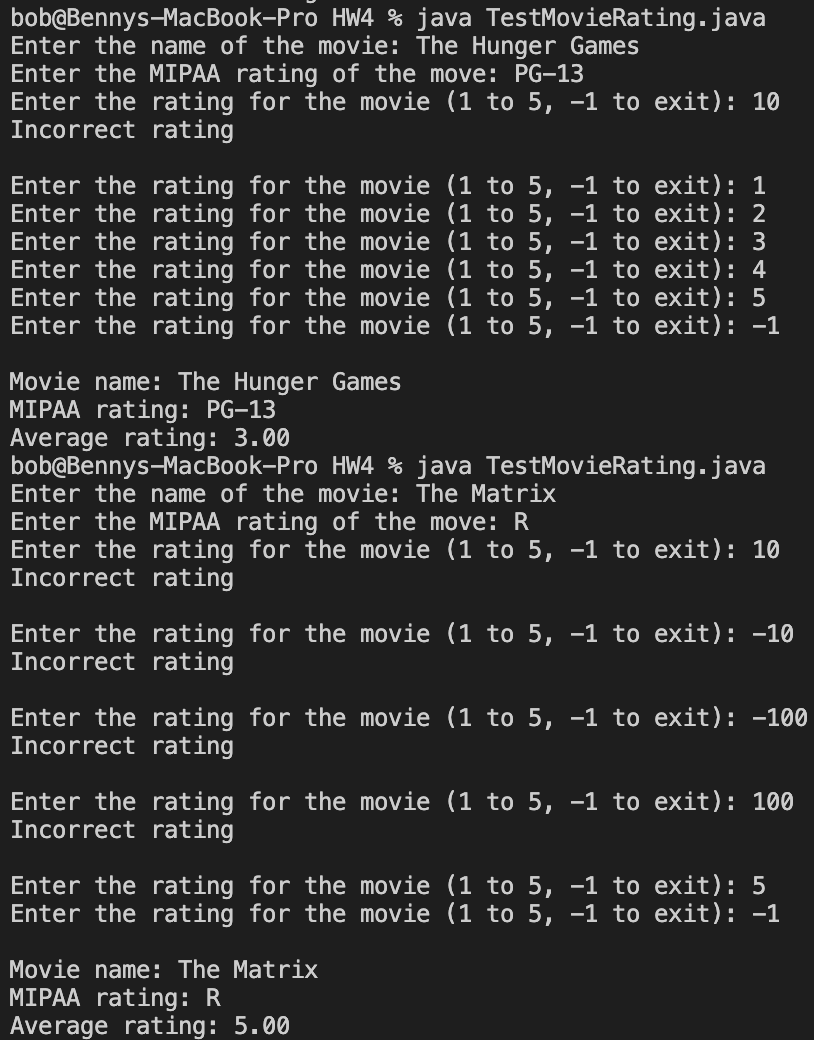
\includegraphics[scale = .65]{test1-2.png}
    \\cont.
\end{center}

\begin{center}
    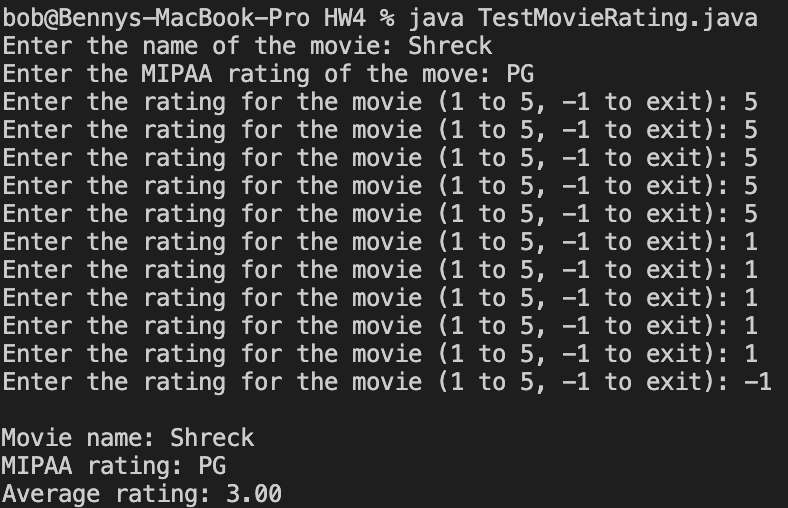
\includegraphics[scale = .65]{test3.png}
\end{center}


\end{document}